\section{Background and Motivation}
\label{SEC:background}

\subsection{The Problem of Environmental Bugs}

\textit{But it works on my machine!} goes the refrain of the tortured
software developer whose application works correctly when executed on a
development computer only to fail once it is deployed.  This occurs with
such frequency that the ``works on my machine'' phenomenon is a well known
source of pain
and frequent topic of discussion
in software and project management
literature~\cite{notreal}.
The problem is so widespread
that FAKESTUDY concluded
that \$XXX are spent annually on efforts to
recall,
fix,
and re-deploy applications
because of all the bugs
that slipped past extensive testing efforts
during development.

Earlier work has demonstrated that environmental bugs, those that occur due
to unanticipated qualities external to an application, are a major source
of such failures.  This fact continues to be reinforced by the regular
appearance of high impact environmental bugs in major pieces of
software~\cite{devzeroroot}.  And it appears that no class of application
is safe with environmental bugs affecting operating systems~\cite{bad},
user applications~\cite{bad} and even web applications~\cite{bad} in the
last year alone!

\subsection{Our Motivating Example}

An initial thrust was made at this problem by Moore et al
when they employed
the Simulating Environmental Anomalies (SEA) technique
on applications' system calls~\cite{crashsim}.
This effort centered on the key insight
that problematic
environmental properties,
known as anomalies, are visible in the
communications between the components that make up an application.
They found that,
once captured,
these anomalies
could be
used to create simulations
that test
an application as if
it had encountered the captured anomalies
in the real world.
But system calls are just part of the story.
This paper documents an effort to augment SEA
so that its proven methodology
can be used to test a broader set of applications.
Our improvements
apply SEA's existing capability
to new bug domains
while maintaining its existing advantages and
dramatically
improving its reach.


\subsection{Why a New Programming Language?}
\begin{figure}
  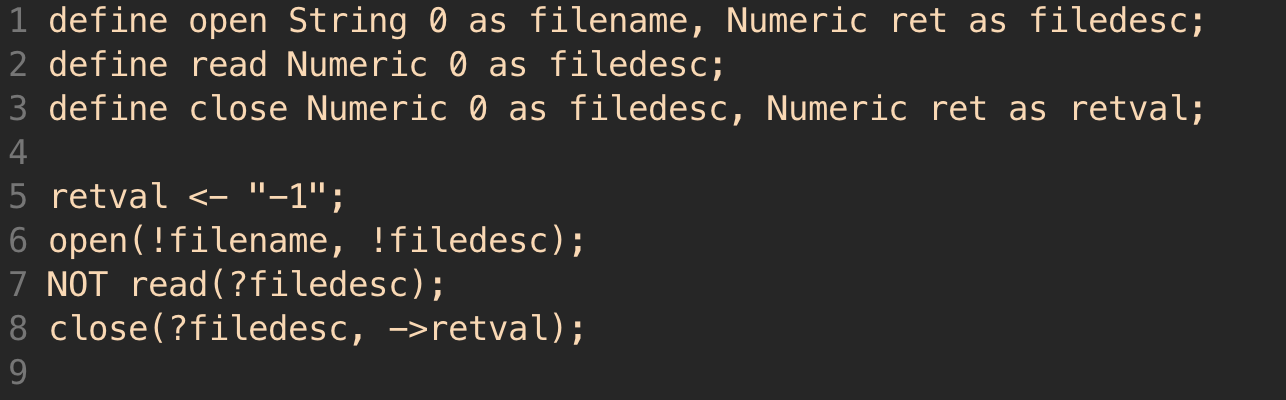
\includegraphics[scale=.50, frame]{images/cslanglisting}
  \caption{A listing of a cslang program.  This program finds situations
  where a program opens a file and closes it without reading from it.  In
  such instances, it modifies the return value close call to be -1,
  indicating failure.}
  \label{fig:cslanglisting}
\end{figure}

\begin{figure}
  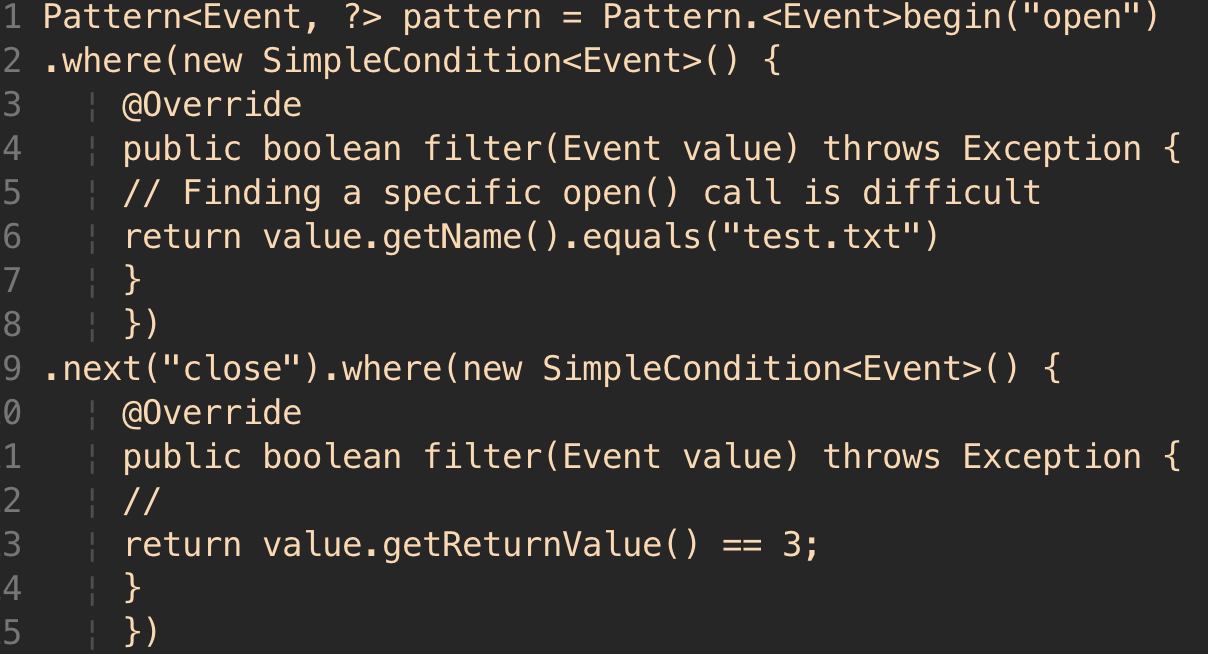
\includegraphics[scale=.50, frame]{images/flinklisting}
  \caption{A listing of an Apache Flink program that does the same thing as the
  cslang program... I need to figure out what comparison stuff to put in
  this caption.}
  \label{fig:flinklisting}
\end{figure}


The decision to create a new programming language was not one we
undertook lightly.  There is a significant amount of work involved in defining,
implementing, documenting, and supporting such a creation.  In this section
we discuss the features we needed for this work and why existing systems fell short
leading to our decision to undertake such an effort.

First, we needed a language that treated state as a first-class citizen.
That is, it must allow the internal contents of events like argument data,
pointer addresses, and return values to be easily captured, manipulated, and
reused in subsequent operations.
This requirement is necessary because,
at a very high level,
the primary purpose of system calls,
function calls,
rpc calls,
or other similar activity
is to allow an application
to gather data from an external module like a library or the operating
system.
As a result, it is frequently useful to be able to store the data returned by
one such action, modify it, and used it in matching actions.
For example, one may store the file descriptor returned by a {\tt
socket()} system call and use it later to match other related,
communication system calls.
This first-class treatment of state served its
purpose well when working with system calls and proved equally useful in
processing input streams from other domains.


% Need to support new event stream formats easily?


\preston{We need to make sure we have given a best effort at shortening and
optimizing code from other languages with which we are making comparisons}

Our second requirement appears to be largely aesthetic at first glance
but there is a
larger purpose -- ease of learning and ease of use.  CSlang offers
improvements over existing languages along two primary fronts.
First, many event processing languages are verbose.
Consider figure~\ref{fig:cslanglisting}  which shows a
CSLang program that matches sequences where an application opens and closes
a file without reading from it.  When such a sequence is found, it is
modified such that the {\tt close()} call returns -1, indicating failure.
The main work of this program is performed in just four lines of CSlang
code.  For comparison, figure~\ref{fig:flinklisting} contains a Java program that
implements an approximation of the same program.  This program does not
perform the return value modification and assumes significant other work
on Apache Flink to allow it to correctly consume a sequence of system calls.
In spite of these shortcomings, comparing the two programs remains
illustrative.  The Flink program is harder to read because it contains a
great deal of boilerplate code
that cannot be avoided due to its dependence on a fully-featured
programming language.  Other work that explores how developers read and
understand (or mis-understand!) code has shown that such constructs obscure
a programs meaning, harming understanding and maintainability.
In light of this, we believe the benefits of a
new programming language
focused on allowing its users to get a lot of work done
with a small amount of easily-readable code are clear.

The second front involves the CSlang's programming paradigm.
While other event processing languages tend toward a functional or
declarative programming,
CSlang programs more closely follow an imperative programming style.
We came to this decision because studies
have shown that developers are more likely to be familiar and comfortable
with such a paradigm~\cite{XXXX}.  We believe this will make it easier for
developers to learn the language, foster greater popularity, and, it aligns
nicely with the goals presented in our motivating example.

Our final requirement is, perhaps, the most important.
We want CSlang programs to be capable of more than simply matching
a pattern of events and indicating that it has occurred.
Our review of the work on the SEA technique has shown that the ability to
{\textit modify} is central to forcing an application into situations where
it may fail rather than only passively monitoring for it to perform
problematic sequences.  While the feature-rich nature of several related
languages and libraries means it is likely possible to modify and output
incoming events it is by no means a straightforward and ergonomic experience.

\preston{Some sort of concluding paragraph?}
